In this section we will be exploring data that can be commonly found in the real world.
While there are infinitely many ways to present and store data, understanding common use cases will allow us to tailor
features specifically for more common formats, and will help with creating realistic simulations in our testing.

Finding every type of commonly used data is futile, so we will attempt to approach several sectors that have a heavy
concern with data, and take a high level overview of the datasets they deal with.

The purpose of this section is to find general types of data that may have to be accounted for, as a consequence, we
will be ignoring specific features of datasets, or datasets driven by events (such as economy data being affected by a
recession, or climate data being affected by global warming).
Once a complete product is produced, a next step could be to take the previously mentioned ignored features of the
analysed datasets, and create specific implementations that account for them.

This can then be used to assign metadata without requiring provided context - e.g.: If we are given unidentified
temperature data, we could suggest adding a metadata tag linking it to our knowledge of how climate temperatures are
modeled.

\subsection{Trading}

Trading is a very data focused profession, predicting trends requires careful analysis of previous data and its effect
on the market.
For this section, we'll look at some of the more common commodities that are traded, and important data sets that are
explored for them.

\subsubsection{Energy}

Energy trading focuses on commodities that generate electricity.
Predicting fluctuations in energy prices requires analysis of data that can affect supply or demand of electricity.

The first data set we will explore is weather.
Typically weather will have a direct effect on energy prices, specifically, lower temperatures cause direct increase
in prices - leading to higher prices in the winter.


\begin{figure}
    \centering
    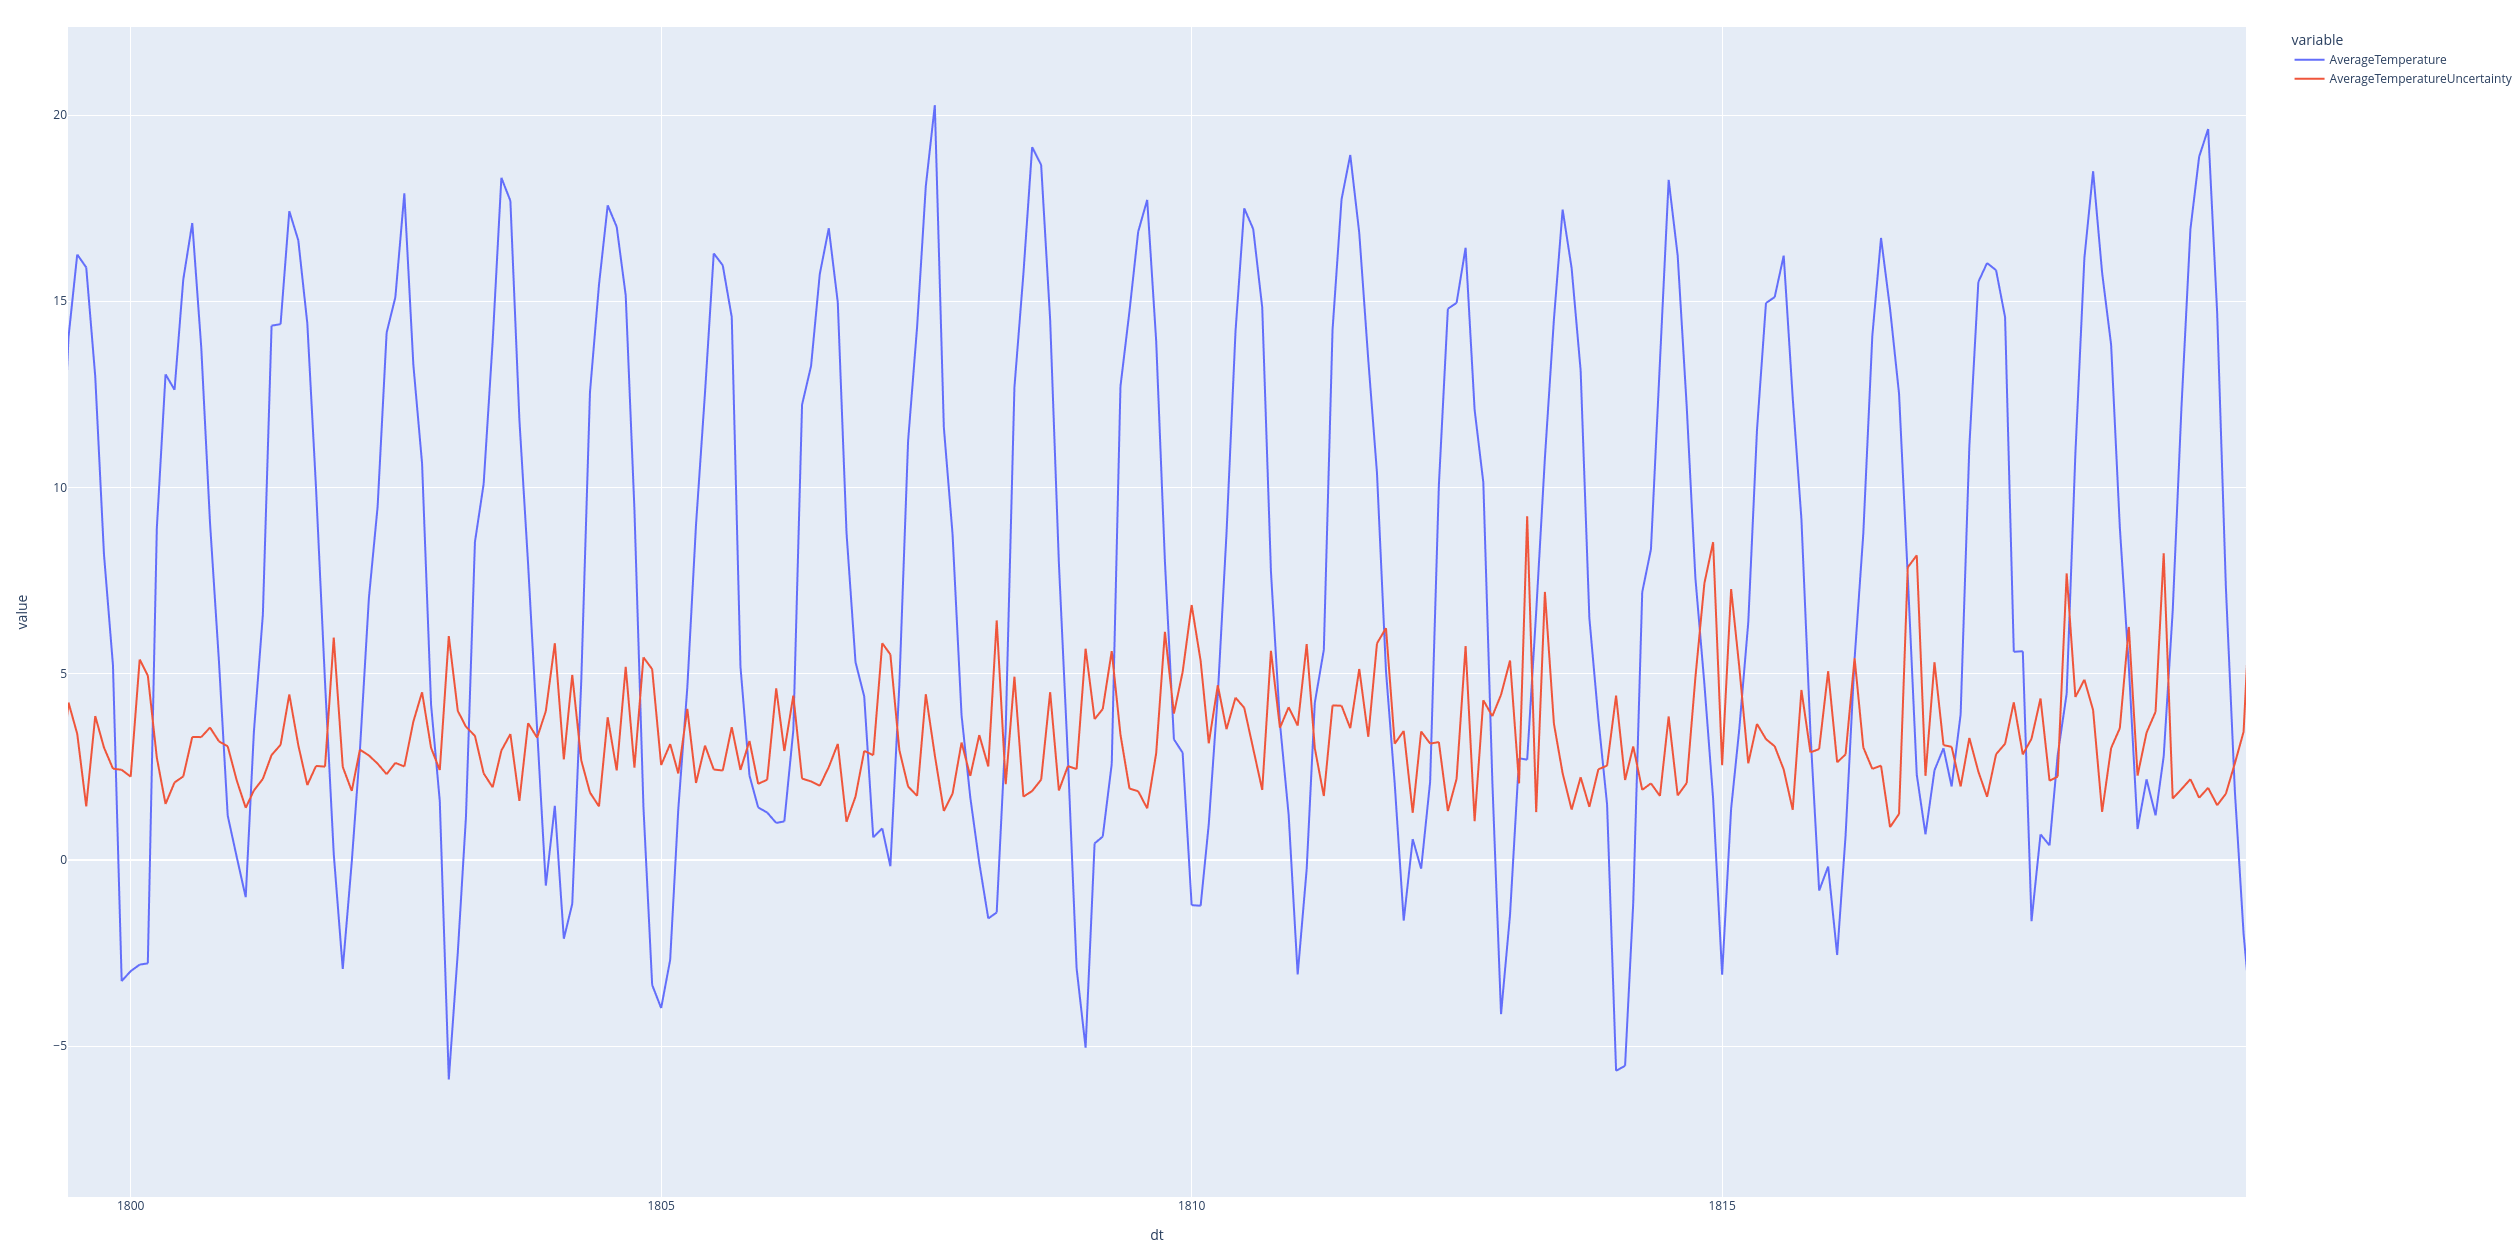
\includegraphics[width=12cm]{figures/real_data_examples/cph_average_temp}
    \caption{The average temperature in Copenhagen over a period of 20 years}
    \label{fig:real_data_climate_cph}
\end{figure}

In figure~\ref{fig:real_data_climate_cph} we plot average temperatures over 20 years - sourced from~\cite{KaggleTemperature}
we can see that temperature very reliably follows a repeating pattern that we could model as a sin wave.

\subsubsection{Currencies}

Trading currencies involves holding a currency that is predicted to increase in value relative to other currencies,
this requires analysis of data that is expected to affect the strength of a currency.

Our first focus point is inflation, as it is well understood concept with easy to model data.

\begin{figure}
    \centering
    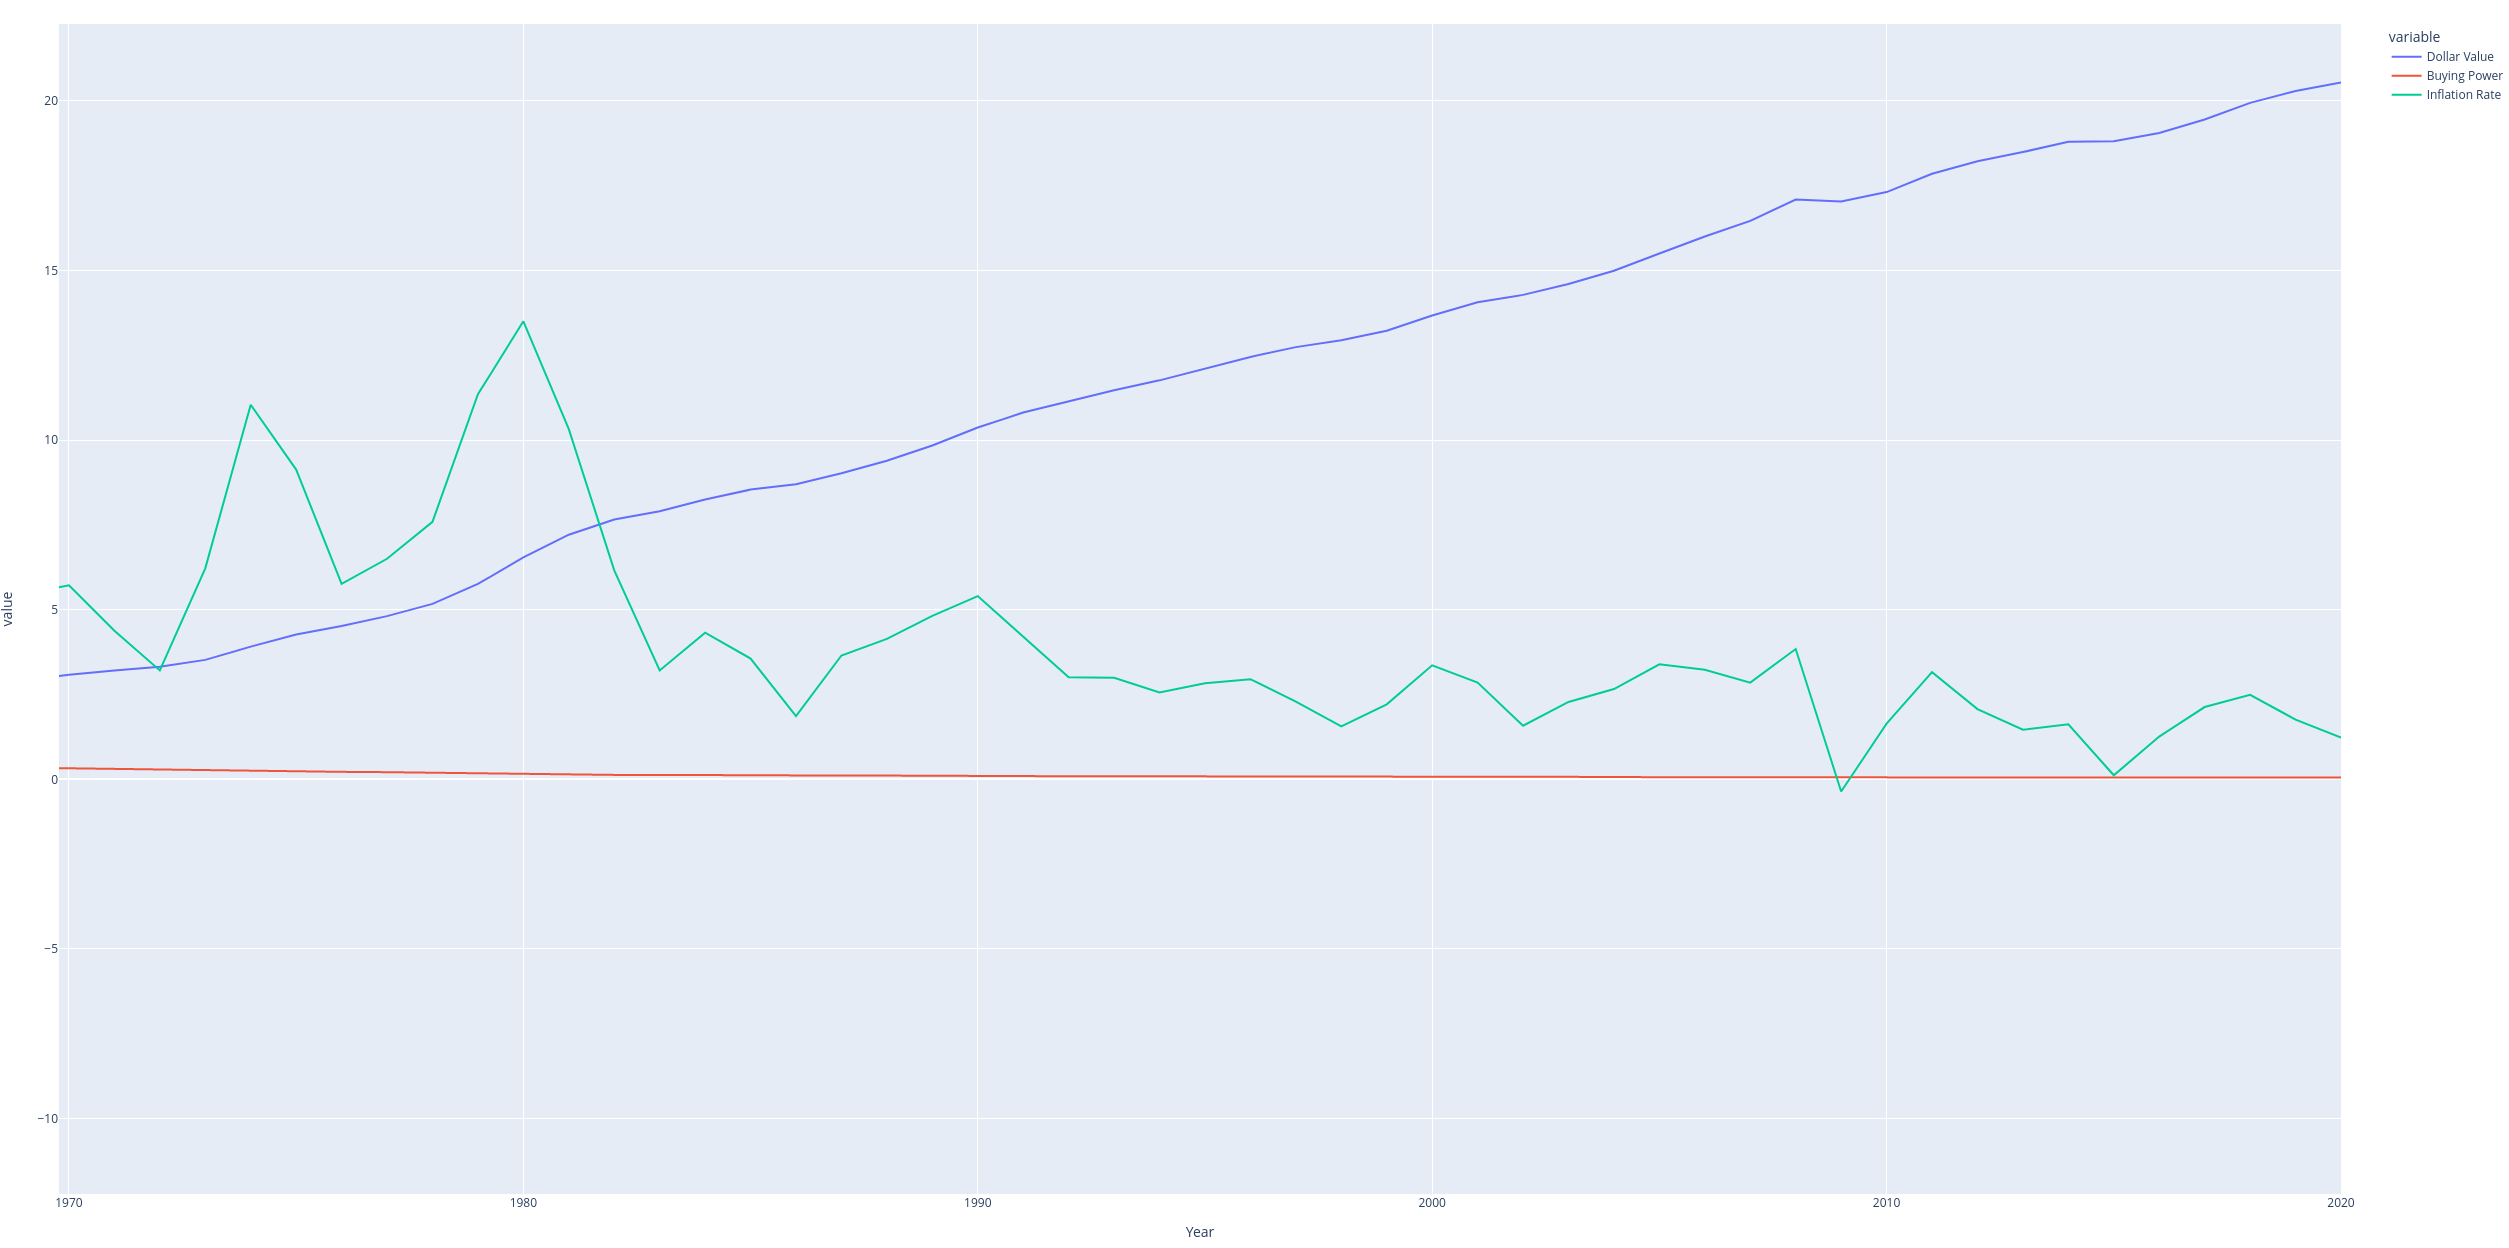
\includegraphics[width=12cm]{figures/real_data_examples/dollar_value_statistics}
    \caption{The buying power of a dollar between 1970 and 2020}
    \label{fig:real_data_inflation}
\end{figure}

In figure~\ref{fig:real_data_inflation} we plot the buying power of the dollar retrieved
from~\cite{officialdataCPIInflationUS}, which can be roughly modeled as a linear graph.
Looking at larger period ranges breaks the pattern that we've established, as specific events have led to drastic
changes before 1970, and in recent years.
It is important to remember here that our goal is not to model specific data sets, for our purposes, we will consider
these changes as simply features of this specific dataset, which may be adressed in more specialised implementations of
our software.

\subsection{E-Commerce}

Companies specialising in E-commerce use data to understand their customers needs, in-depth tracking leads to very large
dumps of various statistics, in this section we will try and identify the types of data that are considered more useful.

\subsection{Medicine}

\subsection{Reflections}

Unfortunately when attempting to research real world data, we found that open source data sets are difficult to procure.
For the purposes of simply finding data to model, we believe we have found enough varied and popular datasets to
create a usable general application, however it is very apparent that more in-depth research would be required to build
specialised metrics.


To recap, the datasets we believe are plausible and useful to model are as follows:

\textbf{Linear data}: Can be used to model anything that increases in a linear fashion in relation to counters or time.
We observed this in currency data, where inflation increases relatively linearly against time.

\textbf{Repeating wave patterns}: Can be used to model anything that maintains an alternating pattern.
We observed this in temperature data, where average temperatures remain similar during the same parts of the year.